%!TEX root = ../Abschlussbericht_Schimmeliger_Keller.tex
%
%  Hochschule für Technik und Wirtschaft Berlin --  Projektabschlussbericht
%
% Kapitel 2 - Vorbereitung und Konzeptentwicklung
%
%

\chapter{Projektplanung} \label{Projektplanung}
\section{Pflichtenheft} \label{Pflichtenheft}

Auch wenn wir in erster Linie ein Produkt aus freien Inhalten entwickeln wollen, müssen wir an einigen Stellen den Kompromiss zwischen freiem Inhalt und Entwicklungsaufwand eingehen, da wir in der zeitlichen Ressource begrenzt sind.
Im Zuge der Projektplanung haben wir eine Umfrage durchgeführt, woraus sich unser Pflichtenheft abgeleitet hat.

 \begin{itemize} 
 	\item \textbf{Anschaffungskosten:} Unser Persona möchte maximal 40 Euro in dieses Projekt investieren, um einen funktionsfähigen Funksensor zu erhalten. 
 	
 	\item \textbf{Laufende Kosten:} Um die laufenden Kostn gering zu halten, soll der Funksensor möglichst stromsparend und wartungsarm sein. Die Hardware sollte ihren Strom über einen Akku bzw. eine Batterie beziehen.
 	
 	\item \textbf{Einsatzgebiet:} Da der Sensor am Mikrocontroller im Bereich von -40°C\dots80°C arbeitet und auch in Gebieten mit einer relativen Feuchtigkeit von bis zu 100\% zum Einsatz kommen soll, muss das fertige Endprodukt mindestens diesen Anforderungen entsprechen. Die Entwicklung eines Gehäuses erfolgt aber erst nach Erreichen der Serienreife.
 	
 	\item \textbf{Datenschutz:} Der Endnutzer möchte selbst bestimmen, ob und mit wem er seine gesammelten Daten teilt. Des weiteren möchte er selbst bestimmen, ab welchem Zeitpunkt/Schwellwert er über den aktuellen Datenstand informiert wird.
 
 \end{itemize}


\subsection{Vorgangsmodell} \label{Vorgangsmodell}
Scrum ist ein Vorgehensmodell im Projektmanagement, welches seinen Ursprung in der Softwareentwicklung hat.
Der Ansatz von Scrum ist das systematische Sammeln von Erfahrungen (empirisch), das kontinuierliche weiterentwickeln bestehender Module (inkrementell), sowie dem mehrfachen Wiederholen gleicher oder ähnlicher Prozesse (iterativ) und basiert auf der Erkenntnis, dass viele Entwicklungsprojekte zu komplex sind, um sie in einem vollumfänglichen Plan fassen zu können, was wiederum den Grund hat, dass wesentliche Teile der Ursprungsanforderung bzw. deren Lösungsansätze zu beginn unklar sind.

Ein weiteres Merkmal von Scrum ist, dass neben dem Produkt auch die Planung kontinuierlich verändert bzw. weiterentwickelt, wobei der langfristige Plan, auch Product Backlog genannt, iterativ verfeinert und verbessert wird.

Resultierende Arbeitspakete werden zyklisch in sogenannten Sprints detailliert formuliert und in einem Detailplan, auch Sprint Backlog genannt, zur Bearbeitung abgelegt, sodass diese, fokussiert auf die aktuelle Problemstellung, abgearbeitet werden können.

Ziel ist dabei eine schnelle und kostngünstige Entwicklung hochwertiger Produkte, wobei die jeweiligen Anforderungen aus der Anwendersicht formutliert werden.

\begin{figure}[h]
	 \centering
	 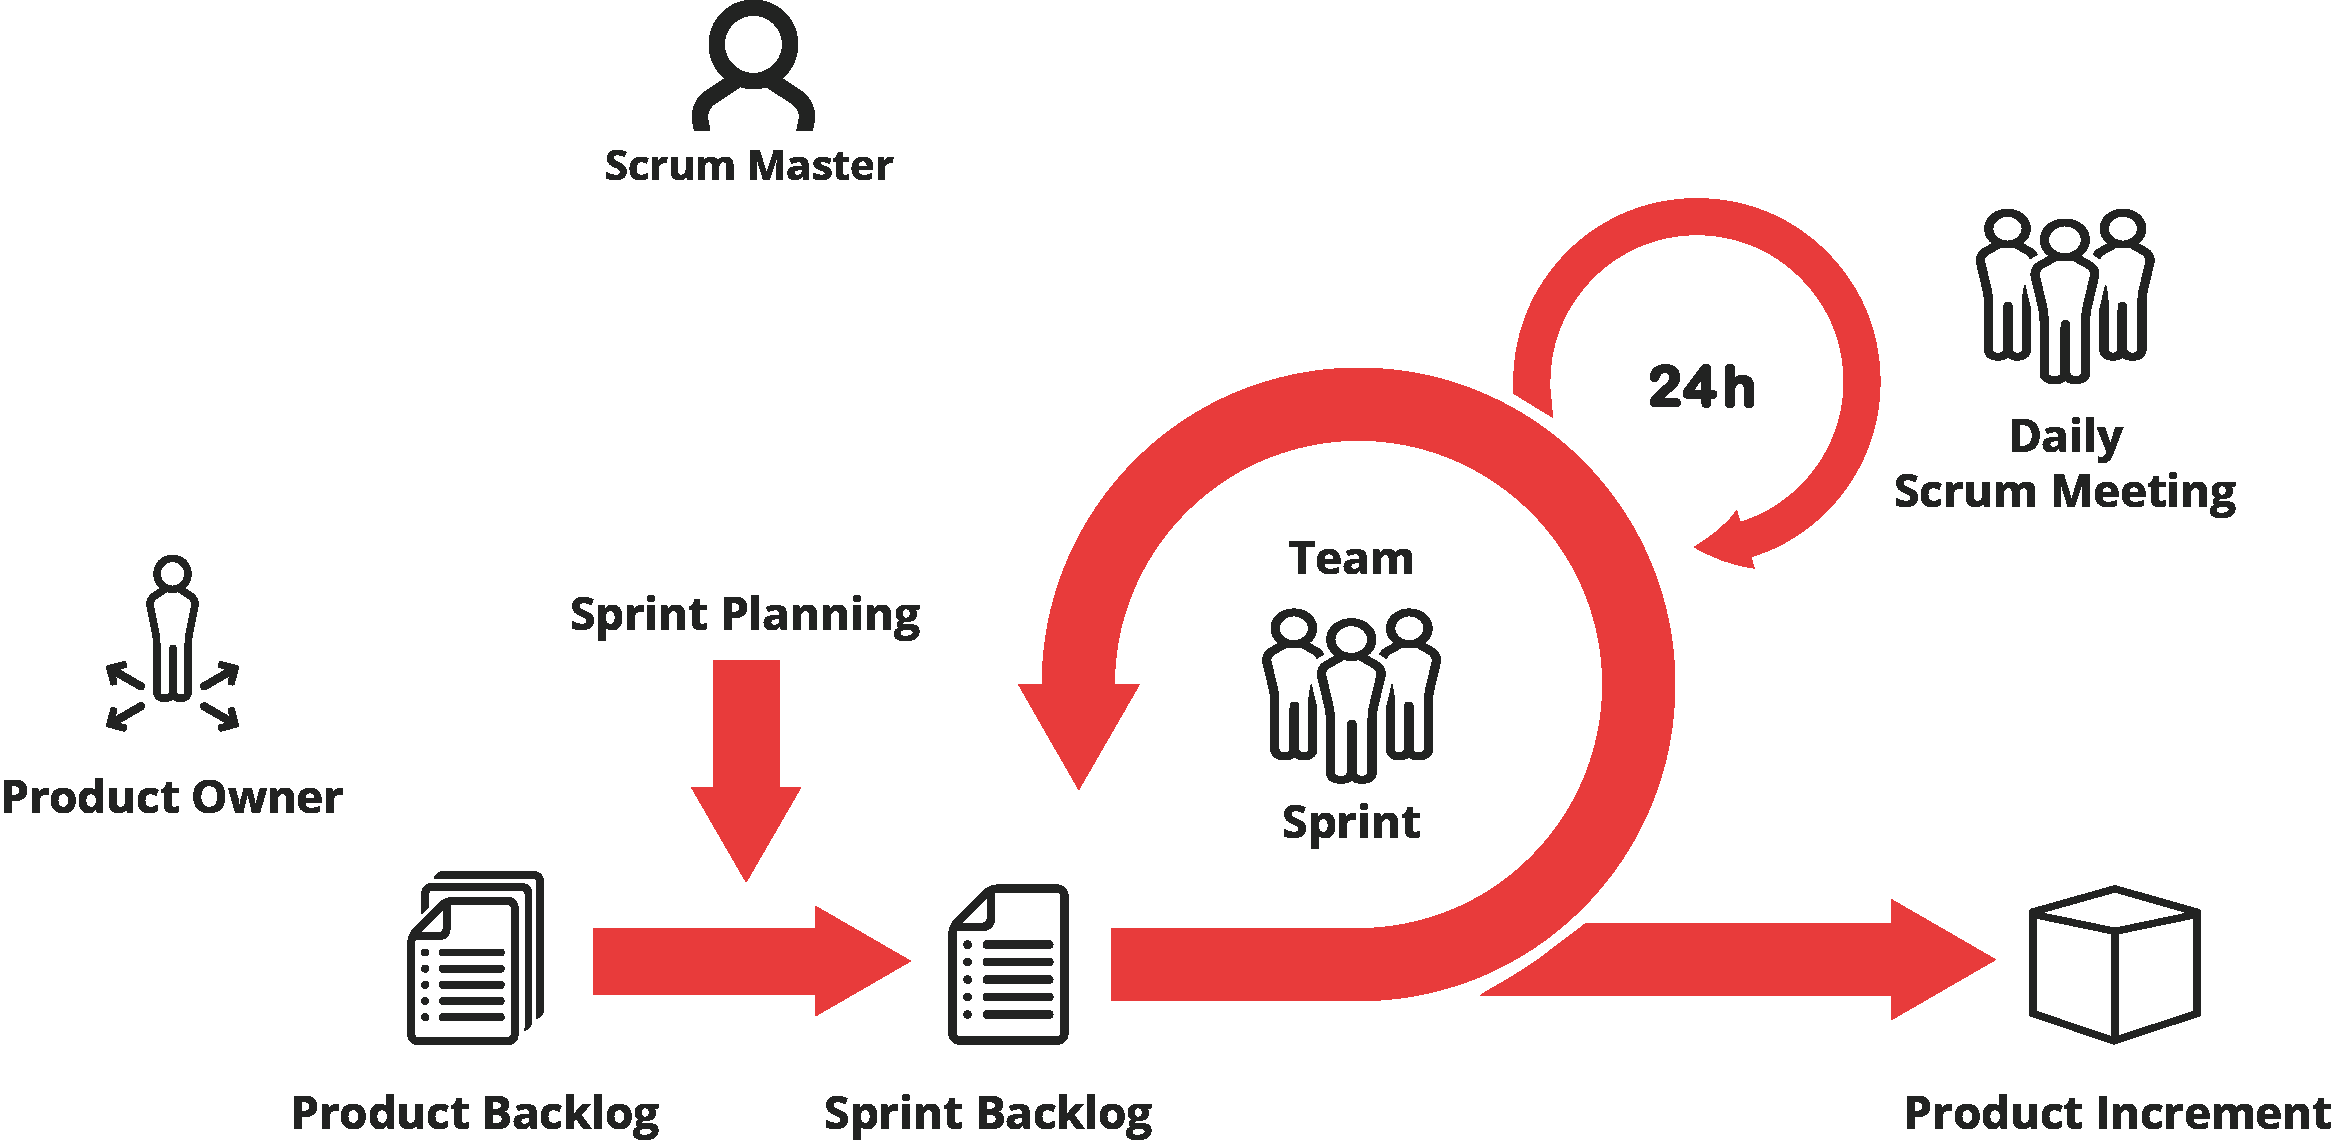
\includegraphics[width=0.8\textwidth]{pictures/scrum}
	 \caption[Agiles arbeiten mit Scrum]{Agiles arbeiten mit Scrum\cite{scrum2018}}
	 \label{fig:scrum}
\end{figure}

Die Verantwortlichkeiten liegt beim sogenannten Scrum-Team, welches sich aus folgenden Rollen ergibt:
\begin{adjustwidth}{-1in}{-1in}% adjust the L and R margins by -1 inch
	\begin{center}
		\begin{tabular}{ ccc }
			\toprule
			{Rolle} & {Besetzung in unserem Projekt} & {Anmerkung}\\

			\midrule
			{Product Owner} & {HTW Berlin} & {Vertreten durch Prod. Dr. Thomas Scheffler}\\
			{Scrum Master} & {-} & {-}\\
			{Projektmanager} & {Sidney Göhler} & {-}\\
			{Scrum Team} & {Sidney Göhler, Ilja Buschujew} & {-}\\
			\bottomrule
		\end{tabular}
		\captionof{table}{Verantwortlichen im Scrum-Team} \label{tab:scrumverantwortung} 
    \end{center}
\end{adjustwidth}


\newpage

\subsection{Projektstruktur} \label{Projektstruktur}

Aus den uns gesetzten Pflichten, haben sich für uns die folgende Projektstruktur grob herauskristalisiert, welche im laufenden Prozess immer weiter in Arbeitspakete verfeinert wurde.


\begin{center}
	\begin{figure}[h]
		 \noindent\makebox[\textwidth]{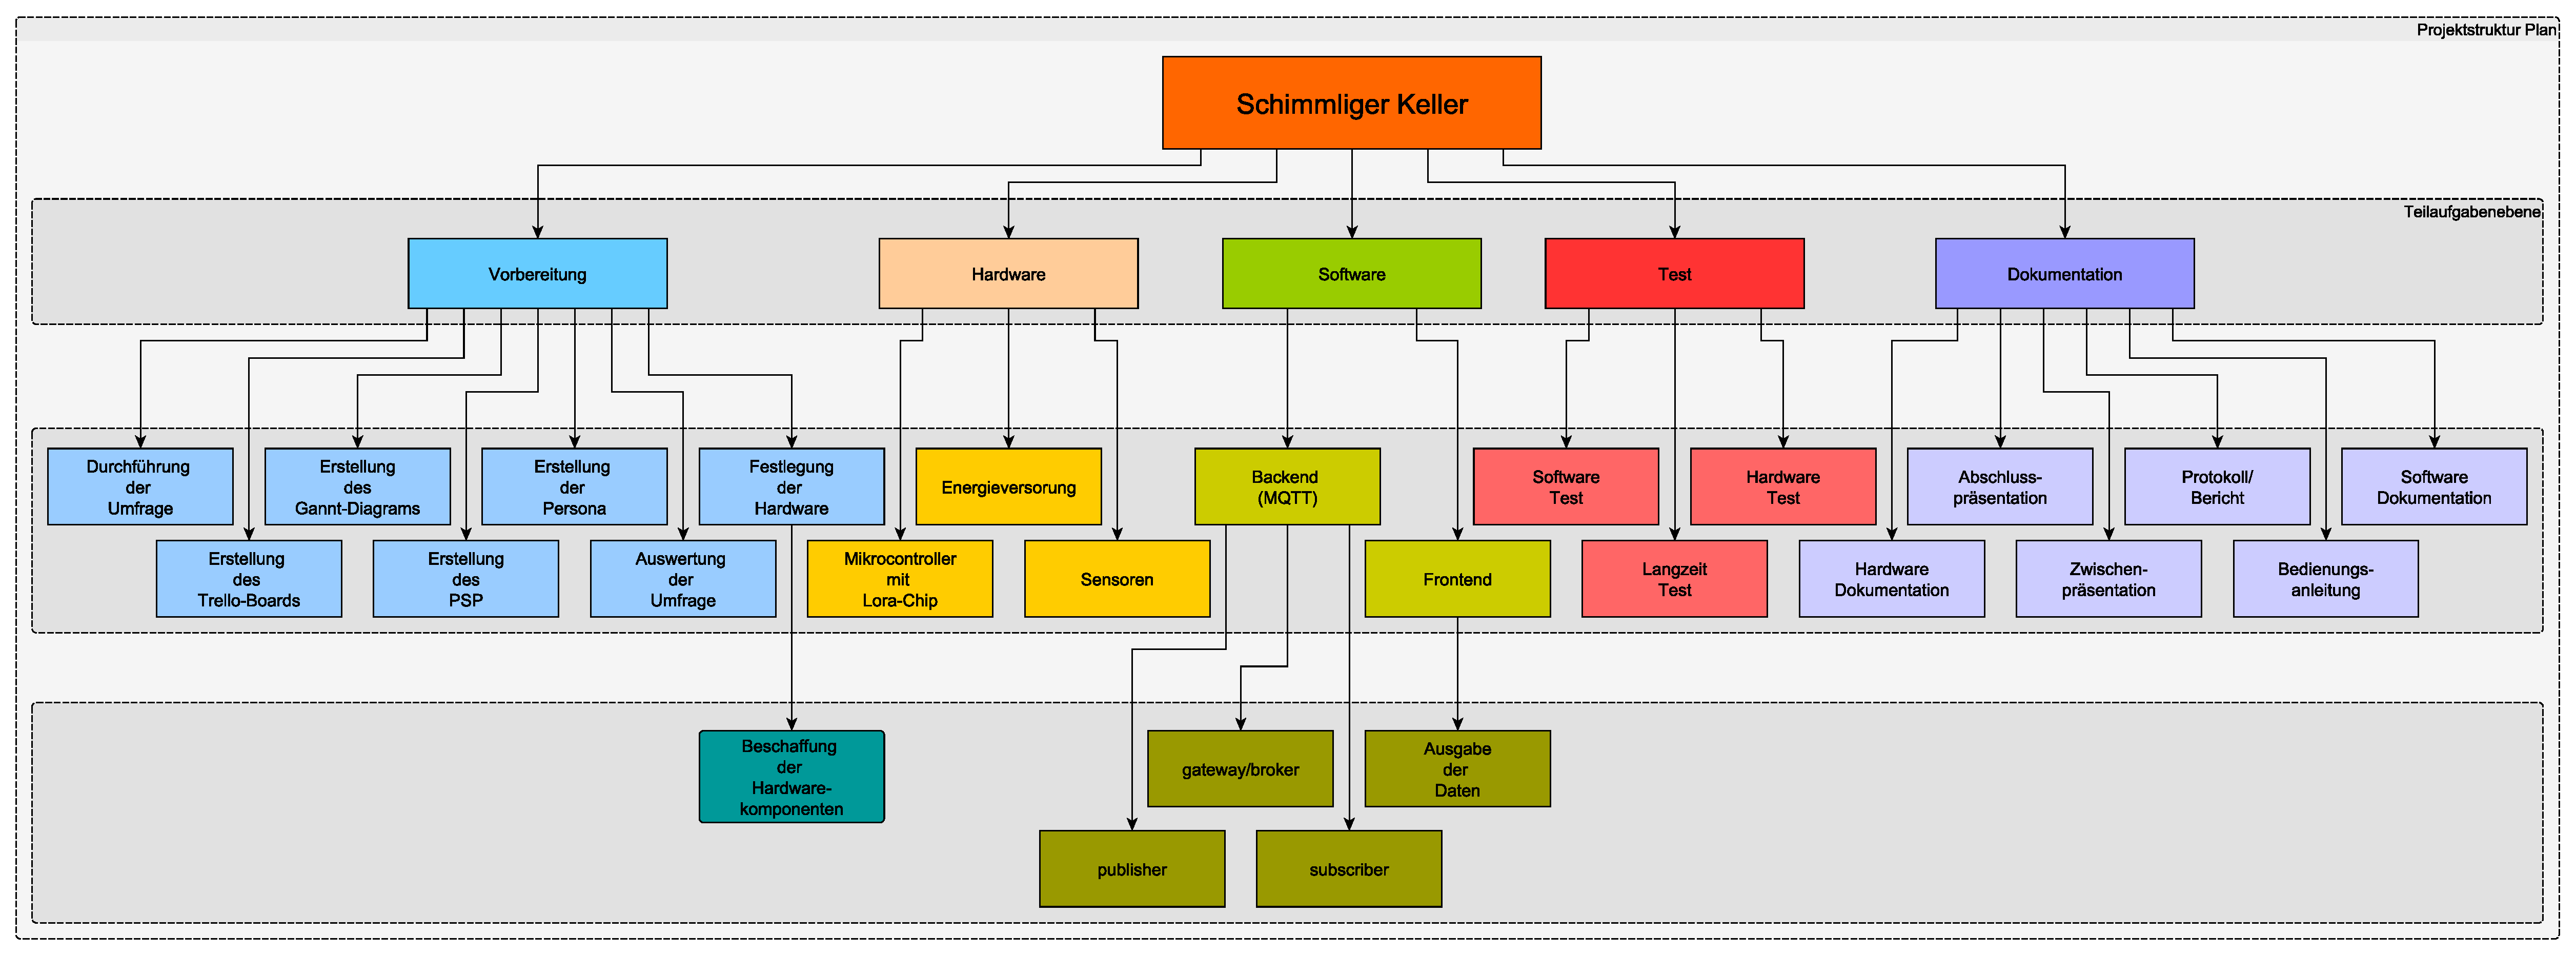
\includegraphics[width=1.2\textwidth]{pictures/PSP}}
		 \caption[Projektstrukturplan]{Projektstrukturplan} 

	\end{figure}
\end{center}

Mithilfe des Projektstrukturplanes ließen grob die einzelnen Arbeitspakete ableiten, wobei diese sich, wie bereits erwähnt, immer weiter verfeinert haben. Der enstehende Aufwand ließ sich zu Beginn noch nicht richtig abschätzen, dennoch konnten wir einen groben Zeitplan für die einzelnen Meilensteine abschätzen.

\newpage

\subsection{Zeitplanung} \label{Zeitplanung}

\begin{center}
	\begin{figure}[h]

	 \noindent\makebox[\textwidth]{
\includegraphics[width=1.3\textwidth]{pictures/zeitplanung}}
	 \caption[Übersicht unserer Zeitplanung]{Übersicht unserer Zeitplanung}
	 \label{fig:zeitplanung}
	\end{figure}
\end{center}

Illustriert wird unsere grobe Zeitplanung zu Beginn des Projektes. Wir wollten aufgrund unserer agilen Arbeitsweise nur grobe Zeiträume definieren. Wie sich schlussendlich herausgestellt hat, haben manche Teilaspekte länger, andere wiederum kürzer gerdauert.\\



\newpage
Nachfolgend wird eine tabellarische Übersicht unserer Zeitplanung aufgeführt, wobei wir die Daten aus unserem Trello-Board entnehmen:\\

\begin{adjustwidth}{-1in}{-1in}% adjust the L and R margins by -1 inch
	\begin{center}
		\begin{tabular}{ ccccc }
			\toprule
			{Vorgangsname} & {Anfang} & {Ende} & {Bearbeiter} & {Arbeitszeit}\\

			\midrule
			\multicolumn{5}{c}{\textbf{Vorbereitung}} \\
			{Sichtung der Quellenlage} & {22.10.2021} & {11.02.2022} & S + I & 20h\\
			{Erstellung Trelloboard} & {22.10.2021} & {22.10.2021} & S & 30m\\
			{Erstellung eines Git repositories} & {22.10.2021} & {22.10.2021} & S & 30m\\
			{Erstellung des PSP} & {29.10.2021} & {29.02.2022} & I & 2h\\
			{Erstellung Zeitplan} & {01.11.2021} & {04.11.2022} & S & 2h\\
			{Erstellung/Durchführung der Umfrage} & {05.11.2021} & {05.11.2021} & S + I & 2h\\
			{Festlegung/Beschaffung der Hardware} & {15.11.2021} & {01.12.2021} & S + I & 3h\\
			{Auswahl/Einrichtung Software IDE} & {01.12.2021} & {20.12.2021} & S + I & 2h\\
			{Auswertung der Umfrage} & {15.11.2021} & {15.11.2021} & S + I & 1h\\
			{Erstellung des Persona} & {15.11.2021} & {15.11.2021} & S + I & 2h\\

			\midrule
			\multicolumn{5}{c}{\textbf{Hardware}} \\
			{Inbetriebnahme der Hardware} & {01.12.2021} & {27.12.2021} & S + I & 2h\\

			\midrule
			\multicolumn{5}{c}{\textbf{Software}} \\
			{µC Management} & {03.01.2022} & {10.01.2022} & S + I & 2h\\
			{Integration der Sensoren} & {10.01.2022} & {04.02.2022} & S & 6h\\
			{Einrichtung einer P2P LoRa-Kommunikation} & {17.01.2022} & {11.02.2022} & S & 6h\\
			{Entwicklung eines MQTT Publishers} & {17.01.2022} & {11.02.2022} & S + I & 2h\\
			{Entwicklung eines MQTT Subscribers} & {17.01.2022} & {11.02.2022} & S + I & 1h\\
			{Einrichtung einer grafischen Schnittstelle} & {10.01.2022} & {11.02.2022} &  I & 2h\\
			{Softwaretests und Bugfixes} & {01.10.2021} & {20.02.2022} & S + I & 6h\\

			\midrule
			\multicolumn{5}{c}{\textbf{Nachbereitung}} \\
			{Vorbereitung der Zwischenpräsentation} & {16.12.2021} & {17.12.2021} & S & 3h\\
			{Vorbereitung der Abschlusspräsentation} & {01.02.2022} & {11.02.2022} & S + I & 6h\\
			{Dokumentation} & {14.02.2022} & {25.02.2022} & S + I & 8h\\
			{Langzeittests} & {20.01.2022} & {11.02.2022} & S + I & 2h\\

			\midrule
			{\textbf{Summe}} & & & & 81h\\

			\bottomrule
		\end{tabular}
		\captionof{table}{Übersicht der Arbeitspakete und Arbeitszeiten} \label{tab:worklog} 
	\end{center}

\end{adjustwidth}

\newpage

\subsection{Kostenaufstellung} \label{Kostenaufstellung}

Auch wenn wir unser Projekt in erster Linie als Freie Software bereitstellen wollen
Aus unseren Anforderungen geht hervor, dass die meisten potentiellen Nutzer möglichst wenig für unser Produkt bezahlen möchten. Wie bei 

\begin{adjustwidth}{-1in}{-1in}% adjust the L and R margins by -1 inch
	\begin{center}

	        \begin{tabular}{cccccc}
			\toprule
			\multicolumn{3}{c}{\textbf{PyCom}} & \multicolumn{3}{c}{\textbf{DIY}}\\

			Name & Anzahl & Kosten & Name & Anzahl & Kosten\\

			\midrule
			LoPy4 & 2 & 38,45 € & ESP32 DevKit & 1 & 9,99 €\\
			Pytrack  & 1 & 40,65 € & Breadboard & 1 & 5,99 €\\
			Antennen-Kit  & 1 & 9,00 € & LoRa Transceiver + Antenne & 1 & 11,98 €\\
			Batterie-Halterung & 1 & 9,00 € & Batterie-Halterung & 1 & 9,00 € \\
			DHT22 Sensor & 1 & 9,99 € & DHT22 Sensor & 1 & 9,99 €\\
			 &  &  & Passive Bauelemente &  & 2,00 €\\

			\midrule
			\textbf{Gesamtkosten} & & 145,54 € & \textbf{Gesamtkosten} & & 48,95 €\\

			\bottomrule

	        \end{tabular}
		\label{}
		\captionof{table}{Kostenaufstellung für das Projekt} \label{tab:kostenaustellung} 
	\end{center}
\end{adjustwidth}

Anzumerken ist hier, dass die Entwicklung des Produktes mithilfe der PyCom Plattfrom zwar deutlich kostenintensiver ist, aber besonders für einen Prototypen doch recht komfortabel, da jeder einzelne Baustein dafür gemacht ist, miteinander zu funktionieren.\\
Tendenziell ließe sich aber mit einem \"Selbstbau\" der Preis um knapp die hälfte reduzieren.\\
Neben der PyCom Plattform existieren noch andere Entwicklungsplattformen, wie z.B. das \textit{TOOGOO WiFi ESP-32 Entwicklungs Board}, welches den LoRa Transreceiver implementiert und teilweise auch schon eine Halterung für Batterien anbietet.\\
Anzumerken ist auch, das der zweite LoPy4 entfallen würde, wenn man sich direkt mittels LoRaWAN an einem Gateway anmeldet und nicht wie wir es gemacht haben, zwei Microcontroller miteinander kommunizieren zu lassen.\\

\newpage


\section{Systemkonzept und theoretische Realisierung} \label{Systemkonzept und theoretische Realisierung}

Nachfolgend wird das Systemkozept und die Realisierung für unser Projekt „Luftfeuchtigkeits-Sensornetzwerk zur zeitnahen Detektion von Wasserschäden auf Basis von LoRa(WAN)“ in Form eines Blockschaltbildes beschrieben. 

\begin{figure}[h]
 \centering
 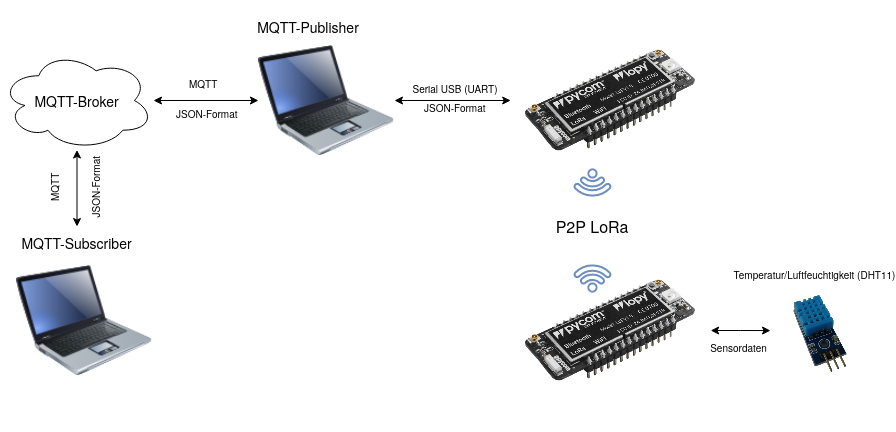
\includegraphics[width=1\textwidth]{pictures/Blockschaltbild_ProNeSy}
 \caption[Systemkonzept für unser Projekt]{Systemkonzept für unser Projekt}
 \label{fig:systemkonzept}
\end{figure}

Für unser Projekt haben wir uns, nach der Beratung mit Prof. Scheffler, dafür entschieden mit den Pycom-Entwicklungsboards zu arbeiten. Diese Boards haben den Vorteil, dass dort schon ein LoRa-Transceiver-Chip integriert ist. 

Da nun sich ein Board mit dem Sensor für die Ausmessung der Luftfeuchtigkeit im Keller befinden soll, wird das andere Board dafür benötigt, um die Sensordaten über LoRa-Kommunikation, in einem Bereich wo es eine Internetverbindung gibt, zu empfangen und über das MQTT-Protokoll an den MQTT-Broker weiterzuleiten, damit andere, die an den Sensordaten interessiert sind, darauf zugreifen können. Als Datenformat wurde sowohl für die Übertragung mittels LoRa, als auch MQTT, JSON verwendet.

Zur Weiterleitung der Sensordaten an den MQTT-Broker wurden die von dem Board empfangenen Sensordaten mithilfe einer UART-Verbindung am Computer ausgelesen und in Form eines Publisher-Clients versendet. Der Subscriber-Client kann nun die jeweiligen Sensorwerte auf den jeweiligen Topics, die er einsehen möchte, empfangen.

Für die Visualisierung der Sensordaten haben wir uns für die Adafruit IO Plattform entschieden\footnote{https://io.adafruit.com/}. Diese Plattform bietet abgesehen von den tollen Visualisierungen der Sensorwerte im Form eines Dashboards, auch einen MQTT-Broker an, den man mit einigen bestimmten Einschränkungen bei der kostenlosen Variante für die eigene Anwendung nutzen kann. 

\begin{figure}[h]
	 \centering
	 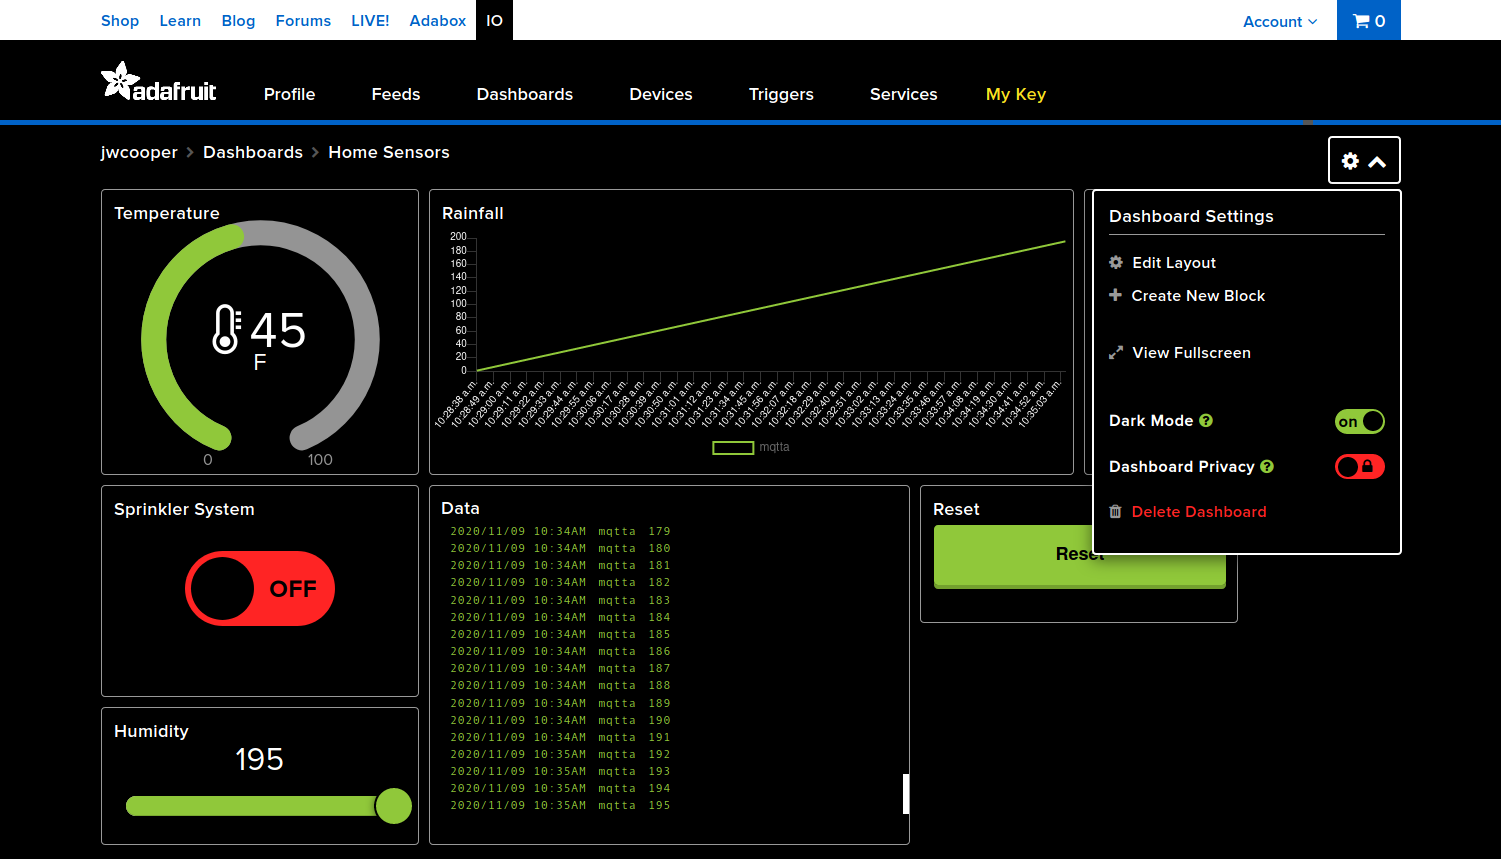
\includegraphics[width=0.8\textwidth]{pictures/adafruitdashboard}
	 \caption[Beispielhaftes Adafruit Dashboard]{Beispielhaftes Adafruit Dashboard\cite{adafruitdash}}
	 \label{fig:adafruitdashboard}
\end{figure}